\chapter{Concepts}
\label{sec:concepts}

\section{Definitions}
\label{sec:concepts:defs}

In the following definitions are given to reason about semantics of implementations of a TeSSLa runtime.
A TeSSLa specification gives a number of transformations over input streams and a subset of the generated streams as outputs.
Streams can be queried for the value they hold at a specific time.

\subsection{Streams}
\label{sec:concepts:defs:streams}

There are two kind of streams: Signals, which carry values at all times and EventStreams, which only hold values at specific times.
EventStreams can be described by a sequence of Events, which hold a value and a timestamp: \((v_1,t_1),(v_2,t_2),\ldots\).
Values can be described by a sequence of changes, which hold a value and a timestamp: \((v_1,t_1),(v_2,t_2),\ldots\).
This shows that the only difference between Signal and EventStreams is given, when we query the stream for it's value:
A Signal will always have a value, an EventStream may return \(\bot\), which denotes, that no event happened at that time.
Because the similarity of Signals and EventStreams in the following we will mainly reason about EventStreams, but most things cam also be applied to Signals.

\subsection{Events}
\label{sec:concepts:defs:events}

Streams consists of events (or changes, which can be modeled the same as events).
There are three Types of Events: Input, Output and Internal events.

Let \(E\) be the Set of valid input events (E for external) and \(e \in E\), where each event carries a value, a timestamp and the
strea, it is perceived on (e.g.\ a function call of a specific function).
Further let \(O\) be the Set of valid output events and \(o \in O\), which have the same properties than input events.

Internal events are mostly an implementation detail, which denotes steps of computation inside the runtime:
Let the Set of valid internal events be \(N\).
Internal events also carry a value and a timestamp, but their stream is implicitly given by the node that produces the event.

\subsection{Functions}
\label{sec:concepts:defs:functions}

A TeSSLa specification consists of functions which manipulates streams and generate new streams.
TeSSLa itself defines a syntax to write a specification, a set of types and a standard library of functions, but an implementation is free to choose the functions it supports.
An example function is \(add(S_D,S_D) \rightarrow S_D\): It takes two Signals, which have to hold values of some numerical type, and produces a signal which holds values of the same type.
The produced stream can either be assigned to a named identifier (think: a variable) or directly be given to another function (function composition).

\subsection{Nodes}
\label{sec:concepts:defs:nodes}

Nodes are the atomic unit of computation for the evaluation of a TeSSLa specification.
A Node implements a single Function, e.g.:\ there is an \emph{AddNode} which takes two input Signals and produces a new Signal.
Therefore a Node is the concrete implementation of a function in a runtime for TeSSLa specifications.

Because Functions in TeSSLa specifications itself depend on other Functions, and these dependencies have to be circle free,
the specification can be represented as a DAG and the Nodes are also organized as a DAg.

% \cleanchapterquote{Innovation distinguishes between a leader and a follower.}{Steve Jobs}{(CEO Apple Inc.)}
% \section{Semantics of TeSSLa functions}
% \label{sec:concepts:semantics_tessla_functions}
% Think of semantics of thinks like add, mrv, etc.
% Can these be defined independent of async/synchronous or for each.
% For synchronous they are partly defined in the TeSSLa spec

\section{Behaviour of different evaluation strategies without timing functions}
\label{sec:concepts:behaviour_without_timing}

For a first step we specify and compare behaviours of different approaches to evaluate TeSSLa specifications without timing formulas,
meaning that only functions, which manipulate values or the presence of events, but not the timestamp of them, are used.
This leads to behaviours that can be easily stated, as seen in the next sections.

\subsection{Ideal synchronous evaluation}
\label{sec:concepts:behaviour_without_timing:ideal}

An ideal system \(I\) for a specification \(T\) is one that consumes an input event \(e_x\) and immediately emits
appropriate output Events \(o_{1,1}, o_{1,2}, \dots , o_{1,x}\) with \(x \in \mathbb{N}_{\ge0}\) and changes it's internal
state \(S\) to save the fact that the event \(e_x\) was received and optionally other properties generated by the
evaluation of the spec that are needed by later computations.

Obviously this approach can not be implemented in practice, but it is a good base to consider equalitys of different approaches.
The Ideal system can be considered as the \emph{Source of Truth}: The Relationship between inputs and outputs it generates
is assumed to be the right evaluation for a given TeSSLa specification.
All other approaches must generate a relationship between inputs and outputs that can be transformed into the one from the ideal system,
or else the different approach is not seen as a valid system for the specification.

The behaviour for a single input can be described by two functions:

\begin{align*}
  \Phi&: S \times E \rightarrow S \\
  \Theta&: S \times E \rightarrow O^*
\end{align*}

The behaviour for multiple inputs is the composition of the functions.

The trace for the implementation \(I\) for a Stream of input events from \(E^*\) is given by the output Stream
from \(O^*\) that is generated by the formulas.

The processing of a series of 3 input events of an ideal system can be visualized like shown in Figure~\ref{fig:chap3:sec_sync:form_sync_processing}.

\begin{figure}
  \begin{flalign*}
    &\text{Timestamp:}  && t_0      &&t_1\                          &&t_2                        &&t_3 &\\
    &\text{Input:}      &&          &&e_1\                          &&e_2                        &&e_3 &\\
    &\text{State:}      && I_0      &&I_1\                          &&I_2                        &&I_3 &\\
    &\text{Outputs:}    &&          &&(o_{1,1}, \dots, o_{1,x})     &&(o_{2,1}, \dots, o_{2,y})  &&(o_{3,1}, \dots, o_{3,z}) &
  \end{flalign*}
  \caption{Example computation of 3 Inputs by an ideal implementation}
\label{fig:chap3:sec_sync:form_sync_processing}
\end{figure}

\subsection{Asynchronous evaluation}
\label{sec:concepts:behaviour_without_timing:async}

An asynchronous system \(A\) for a specification \(T\) is an abstraction of an actual implementation of a runtime.
The actual Implementation consists of multiple Nodes, where each one implements one formula of the TeSSLa specification.
Each Node is run as it's own process and newly generated events are passed as messages to Nodes that work on them.

The asynchronous system doesn't consider a number of implementation details of the actual implementation, e\.g\. the needed computation duration of a Node:
Each Node takes exactly one step to produce a new output based on inputs.

The asynchronous system has a more complex behaviour than the ideal system because Nodes have to wait for other Nodes that are before them
and there are multiple Nodes that can produce outputs.

% It's state is defined by the product of the States of it's nodes, where each node represents a primitive operation in
% the specification and the nodes are organized as a DAG.%TODO glossary
% The output is specified by the concatination of outputs of the nodes that are marked as output nodes in the specification.

In contrast to \(I\) the asynchronous system takes multiple steps to produce an output from an input.
During a step multiple things can happen at once:

\begin{itemize}
  \item A new, external input Event can be consumed by a source in the DAG, which generates an internal event that is propagated to it's children
  \item An internal Node which has at least one new input buffered on its input queue can perform
    it's computation and generate a new internal event, which is propagated to the children of that node, which therefore can compute in the next step.
  \item An output node, which has at least one new input buffered on its input queue, can produce a new output.
\end{itemize}

To reason about the steps $A$ takes while performing a computation, we have to define a schedule of the computations of the nodes.
This schedule has to be fair, otherwise it's possible that no output would ever be created, because the output nodes will never be scheduled.
Such a schedule is given by the following steps:

\begin{itemize}
  \item Number the nodes in reversed topological order
  \item schedule the node with the lowest number that has an input event buffered
\end{itemize}

As shown in Section~\ref{TODO} this is a fair schedule.

Figure~\ref{fig:chap3:sec_async:visual_dag} shows two DAG representations of an asynchronous system where the Nodes A to D are labeled
in a reversed topological order and \(o_1\) and \(o_2\) represents the output channels with that name.
The left system is in it's initial State and an input event \(\langle e_1,t_1\rangle\) is ready to be consumed.
When a node is chosen to compute by the scheduler, only node A is ready, therefore it is scheduled.
The right system is the representation of the next step: Node A has consumed the external event and produced an internal event
\(\langle n_A,t_1\rangle\) which is proppagated to all it's children: Node B and C.
In the next step Node B would be scheduled, because it has the lowest number of any node that can compute (actually it's the only node that can compute at all, because C ahs to wait for the event from B).
After B was scheduled, it would have produced the internal Event \(\langle n_B,t_1\rangle\) which would then be emitted as the output event
\(\langle o_1,t_1 \rangle\).
Therefore the trace of consumed external and produced internal and output events by the system with this specific schedule could be visualized as:
\[
  \langle I_1,t_1 \rangle \langle n_{A1},t_1 \rangle \langle n_{B1},t_1 \rangle \langle o_{1,1},t_1 \rangle \langle n_{C1},t_1 \rangle \langle n_{D1},t_1 \rangle \langle o_{2,1},t_1 \rangle
\]
If there were more than one input event, at this point Node A would be scheduled again, consume the next external event and the following nodes would be scheduled in the same order as before,
extending the trace in an obvious way.

\begin{figure}
  \begin{tikzpicture}
    [pre/.style={<-,shorten <=1pt,>=stealth,semithick}]
    \node (E) at (2,5) {\(<e_1,t_1>\)};
    \node [shape=circle,draw=black] (A) [label=right:4] at (2, 4) {A}
      edge [pre] (E);
    \node [shape=circle,draw=black] (B) [label=left:1] at (0,2.5) {B}
      edge [pre] (A);
    \node [shape=circle,draw=black] (C) [label=right:3] at (4,1) {C}
      edge [pre] (A)
      edge [pre] (B);
    \node [shape=circle,draw=black] (D) [label=right:2] at (4,-1) {D}
      edge [pre] (C);
    \node (o1) at (0,1) {\(o_1\)} edge [pre] (B);
    \node (o2) at (4,-2) {\(o_2\)} edge [pre] (D);
  \end{tikzpicture}
  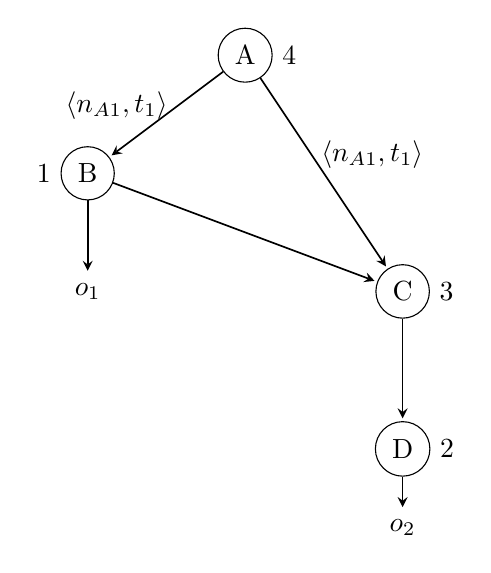
\begin{tikzpicture}
    [pre/.style={<-,shorten <=1pt,>=stealth,semithick}]
    \node [shape=circle,draw=black] (A) [label=right:4] at (2, 4) {A};
    \node [shape=circle,draw=black] (B) [label=left:1] at (0,2.5) {B}
      edge [pre] node[align=left,left,pos=0.6] {\(\langle n_{A1},t_1\rangle\)} (A);
    \node [shape=circle,draw=black] (C) [label=right:3] at (4,1) {C}
      edge [pre] node[align=right,right,pos=0.6] {\(\langle n_{A1},t_1\rangle\)} (A)
      edge [pre] (B);
    \node [shape=circle,draw=black] (D) [label=right:2] at (4,-1) {D}
      edge [pre] (C);
    \node (o1) at (0,1) {\(o_1\)} edge [pre] (B);
    \node (o2) at (4,-2) {\(o_2\)} edge [pre] (D);
  \end{tikzpicture}
  \caption{Visualization of a simple asynchronous system with a reversed topological order.}
\label{fig:chap3:sec_async:visual_dag}
\end{figure}

% TODO Proove equality between different topological orders
% TODO also sth\. about multiple nodes computing at once == (one node at a time + fairness)

\section{Equalitys of different Systems without timing functions}
\label{sec:concepts:equalitys_without_timing}

Based on the described behaviours of the approaches we now can proof the equality of them.

As already stated in Section~\ref{sec:concepts:behaviour_without_timing:ideal} the System \(A\) has to produce an equal
relationship of inputs and outputs as \(I\) to be a valid implementation of the specification.

The equality is shown in two steps: First it is shown, that the computation of \(A\) with a fixed, reversed topological
schedule is equal to \(I\) in Section~\ref{sec:concepts:equalitys_without_timing:ideal_async_topological}.
Afterwards in Section~\ref{sec:concepts:equalitys_without_timing:async_any_async_topological} it is shown that \(A\) with any fair schedule is equal to \(A\) with the fixed, reversed topological schedule,
and therefore equal to \(I\).

\subsection{Asnychronous system with topological schedule and ideal system}
\label{sec:concepts:equalitys_without_timing:ideal_async_topological}

When given a series of input events, \(A\) won't emit the outputs in the same order as \(I\),
but the reversed topological schedule will assure that all outputs that can be produced after consuming a specific input
will be produced before the next Input is consumed as shown in the next sextion.
Therefore, to make the relationship between inputs and outputs the same as the one from \(I\), only the outputs between
each consumed input event have to be reordered.
Stated otherwise: If \(I\) and \(A\) consume exactly one input, they both will produce exactly the same outputs,
only in different order.

The following paragraphs will give a more precise notion of the equality between the systems.

To proof the equality of both systems we have to proof the equality of the traces \(A\) produces, while computing the
outputs, to the traces \(I\) generates.
Let \(e_1, e_2, \dots, e_x\) be the input events both implementations receive.
The trace of \(I\) was shown in Section~\ref{sec:concepts:behaviour_without_timing:ideal} and the traces of \(A\) were shown in Section~\ref{sec:concepts:behaviour_without_timing:async}.

% Due to the asynchronous nature of \(A\) there is no direct mapping from the states of \(I\) to the states of \(A\), because
% \(A\) will compute outputs in a non deterministic order.
% Therefore the equality has to be shown inductive over the possible States \(A\) could reach while computing the outputs.

Let's first reason about the easy case, were only one external event is received:
In this case \(I\) has only two states, \(I_0,\ I_1\) and will only produces outputs once: \(o_{1,1}, \dots, o_{1,x}\).
\(A\) will walk through multiple states, bound by the number of functions in the specification it's implementing.
Because the specification is a DAG, especially has no circles, eventually \(A\) has to finish it's computation, let the
number of steps be \(k\).
Let \(h_{\min}\) be the minimal height of the DAG (the height of the leave with the fewest steps to the Source).
The first output can only be created after \(h_{\min}\) steps and after step \(k\) all outputs have to be created, so that
\(o_{1,1}, \dots, o_{1,x}\) were emitted.
Let the States of \(A\) during the computation be \(A_{0}, A_{1,0}, A_{1,1}, \dots, A_{1,k}\) where \(A_0\) is the initial state.

When taking the first step and \(A_{1,0}\) is reached, the event \(e_1\) is consumed by a source node \(N_A\), which produces
the internal event \(\langle n_{A,1},t_1\rangle\) and distributes it to it's children.
Note that there is no alternative to this bahivour, because there were no prior events and therefore no internal Node
has an event to process on it's input queue, therefore the Source consuming the external event is the only node that can,
and therefore must, compute anything.
Afterwards all Nodes that are direct children of the source that consumed the external event will have one input event buffered and
are able to perform their computation in the next step.

At least until step \(h_{\min}\) every step one or more Nodes, that are no outputs, will perform a computation, therefore
pushing internal events closer to the output nodes.
Somewhere between step \(h_{\min}\) and \(k\) all internal events will reach an output node and produce an output.

A more complex case is when multiple external events are received.

Because the scheduling of nodes of \(A\) is based on the reversed topological order, \(A\) will only consume one new external event and then will schedule internal nodes until all
internal events have reached an output node, only than the next input will be consumed by a source node.
\(I\) will step through a series of States \(I_0, I_1, \dots, I_x\), A on the other hand will step through a Series of
states for each state that \(I\) takes: \(A_0,A_{1,0},A_{1,1},\dots,A_{1,j1},A_{2,0}, \dots,A_{x,j2}\) and generate internal events along those steps.
Based on this behaviour lets define when a State of \(A\) is equal to one of \(I\):
The first states \(A_0\) and \(I_0\) are always assumed to be equal, because no output can be observed and therefore one
can't observe a difference.
A State \(A_{i,j}\) with \(j > 0\) is called equal to a State \(I_{i}\) iff:

\begin{itemize}
  \item The previous state \(A_{i,j-1}\) was equal to \(I_{i}\)
  \item and either
    \begin{itemize}
      \item No new output was generated at state \(A_{i,j}\)
      \item or if a new output \(o\) is created it is equal to one of the outputs of \(I_{i}\) that wasn't generated before
    \end{itemize}
\end{itemize}

A State \(A_{i,0}\) is called equal to a state \(I_{i}\) iff

\begin{itemize}
  \item The previous state \(A_{i-1,x}\) was equal to \(I_{i-1}\)
  \item the input \(e_i\) was consumed at the step
  \item and the States \(A_{i-1,0}\) to \(A{i-1,x}\) together produced the same output like \(I_{i-1}\)
\end{itemize}

Naively speaking the System \(A\) moves through states \(A_{i,0},\dots,A_{i,x}\) while it produces the same outputs as \(I\)
produced when it reached state \(I_i\), and as soon as the last output was produced consumes a new event and thereby takes
state \(A_{i+1,0}\).

Based on this, a series of states \(\vec{A}\) is called equal to a series of States \(\vec{I}\) if each state in \(\vec{A}\)
is equal to a state in \(\vec{I}\).
The System \(A\) is equal to the system \(I\) in regard to a series of inputs \(\vec{e}\) iff all possible series of
states it could take to process \(\vec{e}\) are equal to \(\vec{I}\).

\subsection{Equality of asynchronous systems with different schedules}
\label{sec:concepts:equalitys_without_timing:async_any_async_topological}

When the Nodes of \(A\) aren't scheduled in reversed topological order, the system can consume Inputs before producing all outputs
based on the last consumed input.
Therefore the reordering of outputs and inputs (and internal events) has to be performed over the whole trace, not only between Input events.
Idea: each step is a commutation of two internal events in regard to the rev top order.
=> show commutativity of traces (note: only valid commutations, no two events, where one depends one the other, can be commuted, this is ensured by the scheduling of nodes that have input buffered)

% \begin{figure}[htb]
%     
\includegraphics[width=\textwidth]{gfx/Clean-Thesis-Figure}
%     \caption{Figure example: \textit{(a)} example part one, \textit{(c)} example part two; \textit{(c)} example part three}
%     \label{fig:system:example1}
% \end{figure}


% \begin{figure}[htb]
%     
\includegraphics[width=\textwidth]{gfx w/Clean-Thesis-Figure}
%     \caption{Another Figure example: \textit{(a)} example part one, \textit{(c)} example part two; \textit{(c)} example part three}
%     \label{fig:system:example2}
% \end{figure}

